\section{Results}
\label{sec:results}
Our study demonstrates the efficacy of our methodology in enhancing the visual presentation of objects within 3D reconstructions. As depicted in Figure 1, the unprocessed Panoptic reconstruction exhibits visual artificats and irregularities, while our approach yields smoothed surfaces, facilitating improved recognition through visual observation. Additionally, we observe the sensitivity of our alignment procedure to the instance masks generated by Panoptic. Although the predicted objects maintain smoothness, our alignment algorithm occasionally results in object intersection, as illustrated in \cref{fig:lim}.

\paragraph{Panoptic Reconstruction Training}

We leverage our synthesized dataset to refine the training of the panoptic reconstruction model proposed by \citet{dahnert2021panoptic}.
Initially, we pretrain the 2D encoder, depth estimation and 2D instance prediction with an ADAM optimizer using a batch size of 1 and learning rate 1e-4 for 570k iterations.

The evaluation results for our 2D model compared to the pre-trained model from \citet{dahnert2021panoptic} are presented in \cref{tab:2dresults}.
As illustrated in \cref{fig:qual_panoptic}, our approach shows performance comparable with the pre-trained model. However, it encounters challenges in generating completely clear depth results, occasionally displaying some irregularities.
Despite our efforts, limitations such as time constraints and the relatively small size of our dataset hindered our ability to train a 3D model that achieves performance on par with the pre-trained counterpart. We refer to the future work section in this regard.
\begin{table}
  \centering
  \begin{tabular}{@{}lccc@{}}
    \toprule
     & Depth & Box Class. & Box Regress. \\
    \midrule
    \citet{dahnert2021panoptic} & 0.23 & 3.39 & \textbf{0.092}\\
    Ours & \textbf{0.196} & \textbf{1.3} & 0.149 \\
    \bottomrule
  \end{tabular}
  \caption{Results for joint training of the 2D encoder, depth estimation and 2D instance prediction. For depth we report the $\ell_1$ distance between the predicted and ground-truth depth maps. Additionally we report the $\ell_1$ distance for the regressed 2D boxes and a CE-loss on the box classification.  }
  \label{tab:2dresults}
\end{table}

\begin{figure}[t]
  \centering
  \begin{subfigure}[b]{0.45\linewidth}
    \centering
    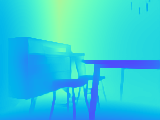
\includegraphics[width=\linewidth]{figs/depth_ours.png}
    \label{subfig:sub1}
   \vspace*{-3mm} % Adjust vertical spacing between the caption and the images
  \caption{Depth map (ours).}
  \end{subfigure}
  \hfill
  \begin{subfigure}[b]{0.45\linewidth}
    \centering
    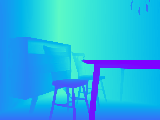
\includegraphics[width=\linewidth]{figs/depth_pan.png}
    \label{subfig:sub2}
   \vspace*{-3mm} % Adjust vertical spacing between the caption and the images
  \caption{Depth map (\citep{dahnert2021panoptic}).}
  \end{subfigure}

  \vspace{0.03\linewidth} % Adjust vertical spacing between rows of figures

  \begin{subfigure}[b]{0.45\linewidth}
    \centering
    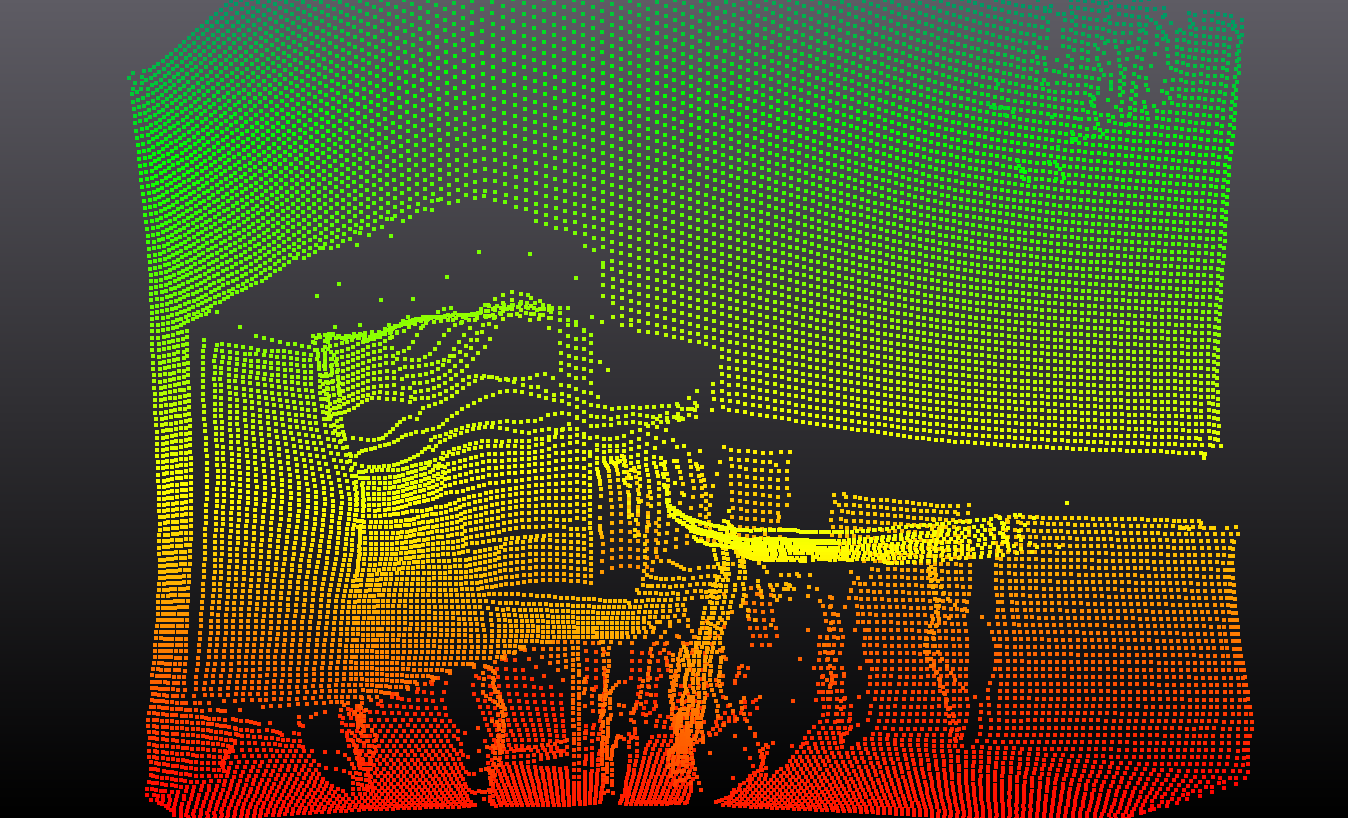
\includegraphics[width=\linewidth]{figs/depthply_ours.png}
    \label{subfig:sub3}
   \vspace*{-3mm} % Adjust vertical spacing between the caption and the images
   \caption{Geometry from depth (ours).}
  \end{subfigure}
  \hfill
  \begin{subfigure}[b]{0.45\linewidth}
    \centering
    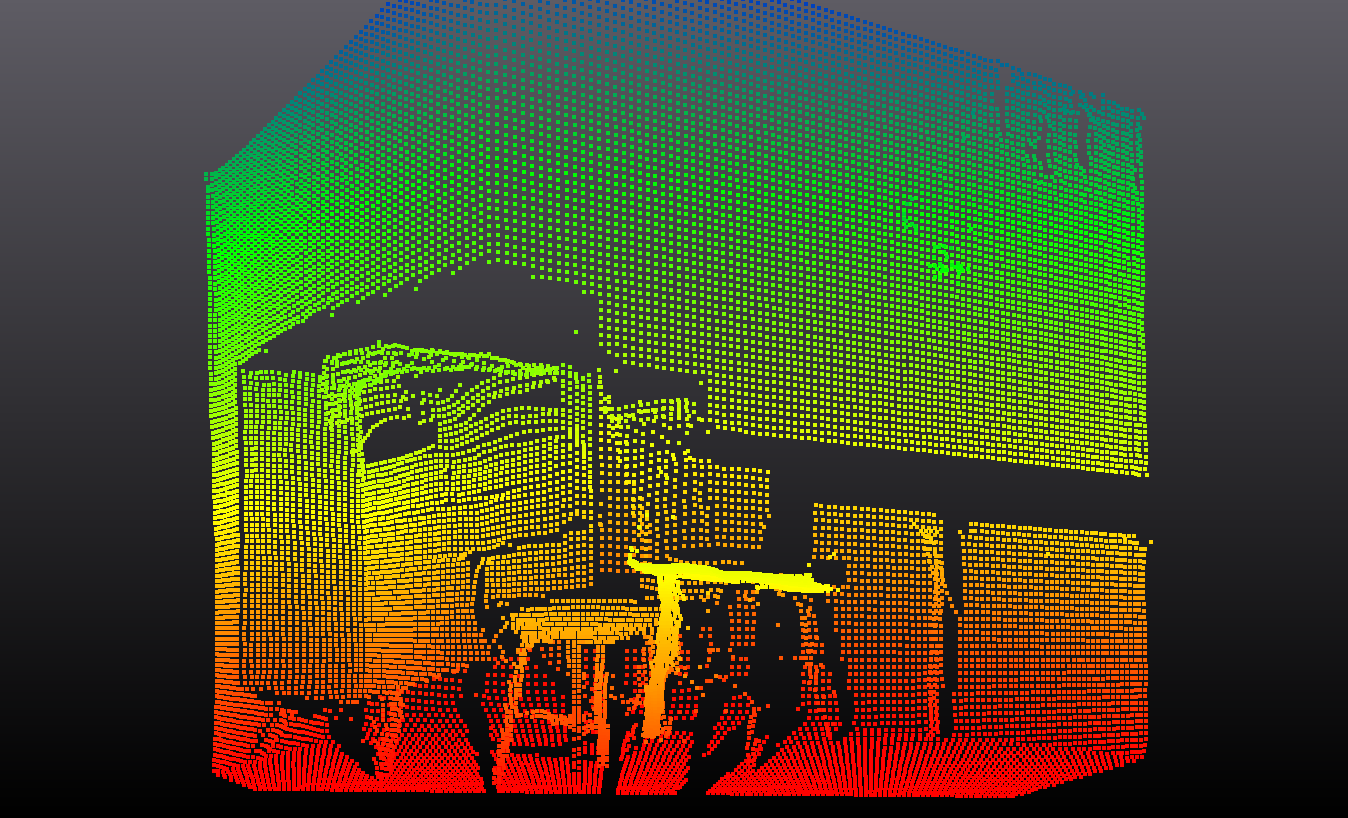
\includegraphics[width=\linewidth]{figs/depthply_pan.png}
    \label{subfig:sub4}
   \vspace*{-3mm} % Adjust vertical spacing between the caption and the images
   \caption{Geometry from depth (\citep{dahnert2021panoptic}).}
  \end{subfigure}

  \caption{2D results from the Panoptic 3D model. Our re-training results (left) vs. results from \citet{dahnert2021panoptic} (right).}
  \label{fig:qual_panoptic}
\end{figure}

\paragraph{SDFusion Fine-tuning}
In order to align SDFusion to the shape distribution of 3D-Front, we fine-tune the model on a subset of the 3D-Future dataset \citep{fu20213e}, which contains the objects used in the scenes of 3D-Front.
We train the model for 12k steps using the original hyperparameters from \citet{cheng2023sdfusion} but with a batch size of 32 (see Figure \ref{fig:finetune}).

\begin{figure}
  \centering
  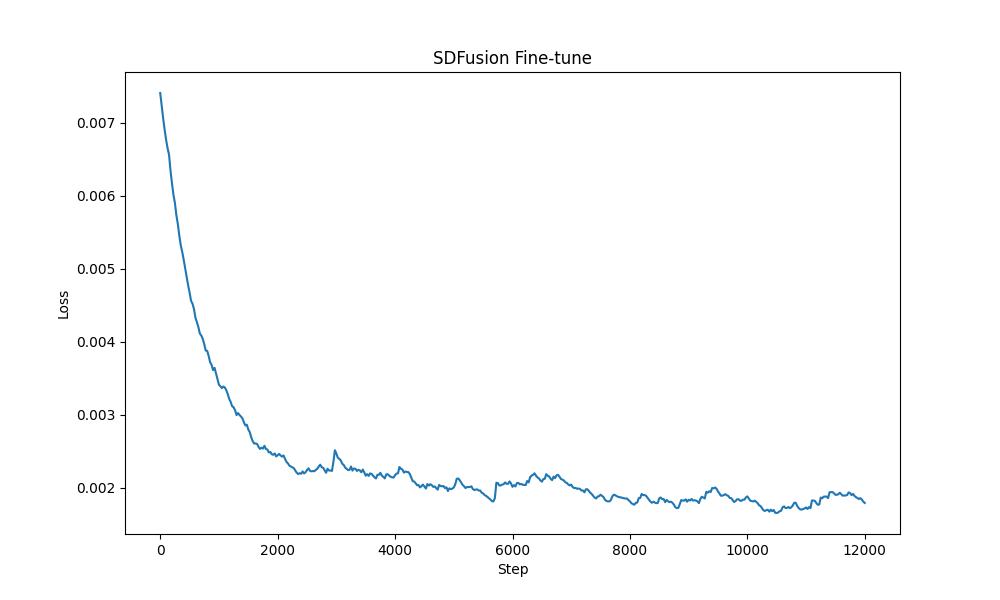
\includegraphics[width=\linewidth]{figs/sdfusion_finetune_loss_plot.png}
  \caption{Loss curve of our SDFusion fine-tune (smoothed).}
  \label{fig:finetune}
\end{figure}

\paragraph{Inference Pipeline}
TODO add visual results
